\chapter{System design}
\label{cha:design}

\begin{figure}
\centering
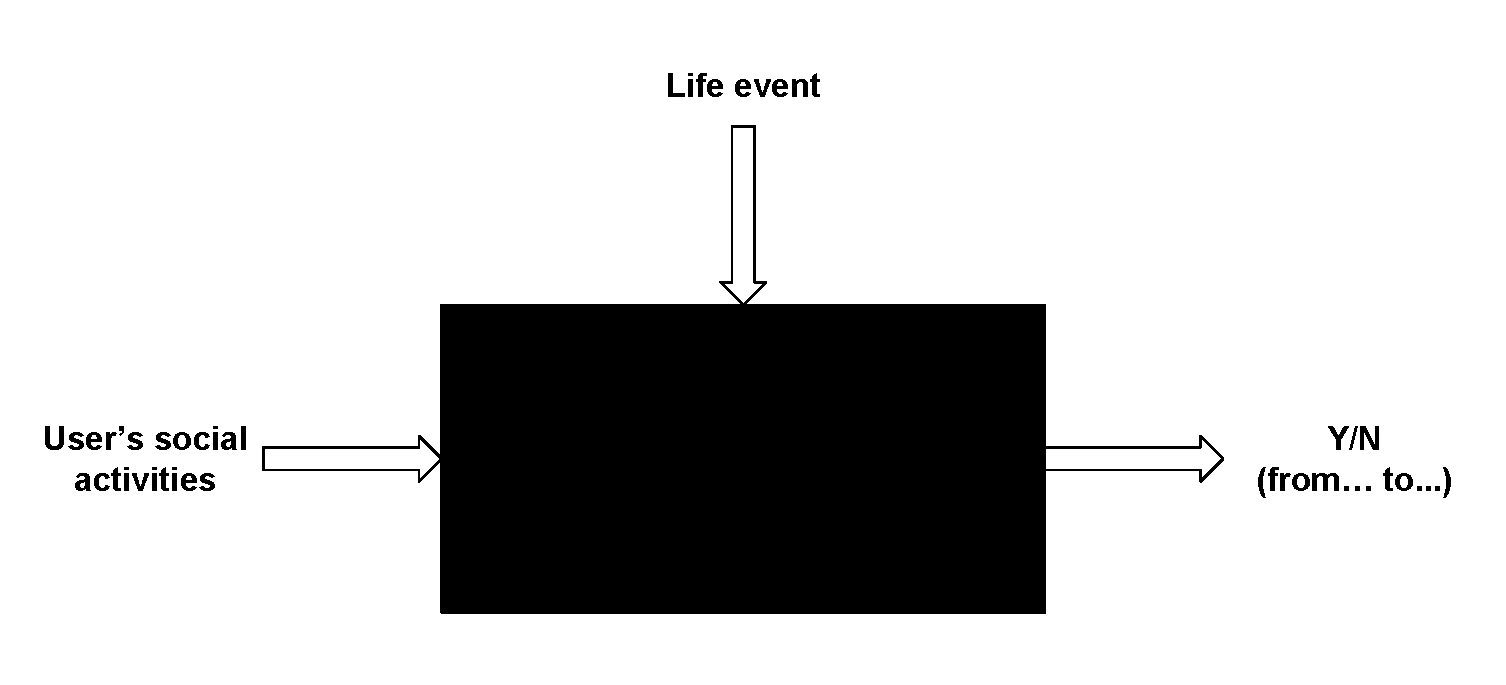
\includegraphics[width=%
0.95\textwidth]{img/bb}
\caption{A black box view of the problem.}
\label{fig:bb}
\end{figure}

In this chapter the design process is presented, starting from the requirements and the description of the working logic. After that, a more schematic view is provided, explaining how the system is designed and how the components work and communicate each other. At the end, the algorithms used to compute the outputs are presented and explained.

Seen as a black-box -- in Figure~\ref{fig:bb} -- the system takes two inputs: all the user's activities in the social networks she is registered in, and a life event to search for, and it returns as output a yes/no answer to the question "\textit{has this user lived this life event?}", with a time reference estimation attached.

\section{Requirements}

The main requirement is that the software solution has to be able to decide whether the user taken into analysis has lived a given life event. The decision has to be taken by analyzing her activities on the social networks she is registered in. The time required to perform this computation should not be long, although data come from an online stream of contents.

Other requirements expect to let the addition of a new user to analyze, or to add and remove a social media account to an already existing user.

The set $S$ of life event that can be searched for should be defined a priori, and it will be: 
\[
S = \{\text{\texttt{Getting married}}, \text{ \texttt{Having children}}\}
\]

\section{Logical components}
\label{sec:logicdescr}

\begin{figure}
\centering
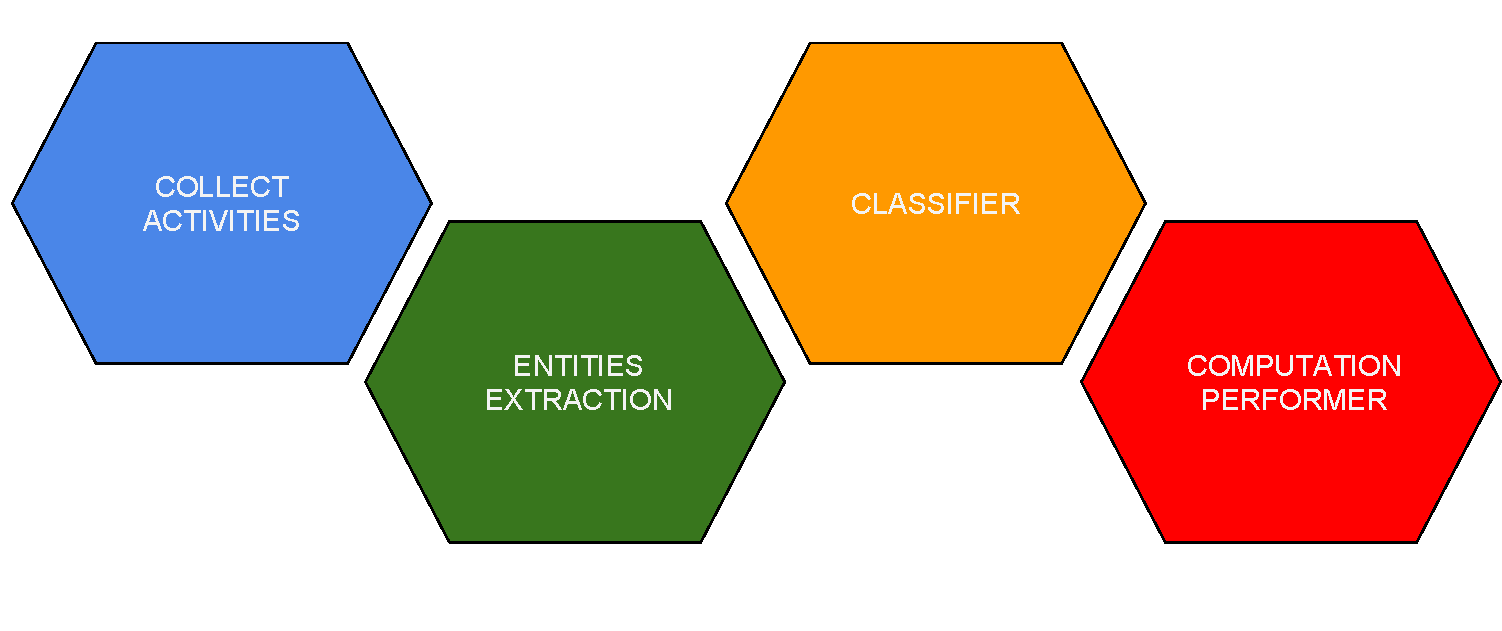
\includegraphics[width=%
0.95\textwidth]{img/Solutiondesign_nutshell}
\caption{The solution design in a nutshell.}
\label{fig:nutshell}
\end{figure}

This section describes the specifications of the logical functionalities of the system. Each functionality is a group of actions whose purpose is to carry out a section of the job required to go from row data - a user identifier - to a piece of information - the answer to the question \textit{"Has this person lived a life event?"}. The steps are the following, as shown in Figure~\ref{fig:nutshell}:
\begin{enumerate}
\item Collect activities from social networks.
\item Extract semantic entities from social network contents.
\item Classify each content.
\item Decide whether the user has lived the life event relying on his/her contents.
\end{enumerate}
Each step relies on what the previous steps do: for example, to execute the third one, the first and the second ones must have already been executed at least once. The number of executions required to perform the entire computation from scratch is probably not the same for each part: in fact, the first two steps are coupled together, and they need to be performed a consistent number of times before fetching an entire user's timeline. Once the whole timeline is downloaded, just a single call for the third and the fourth steps is needed to complete the computation. In the following subsections the logic of the proposed methodology is illustrated, providing a textual description of what each component has to do, of the input, the output and the parameters. 

\subsection{Collect activities}
This part has the goal to fetch user's contents on social networks, using the services for developers offered by the official APIs of each social network. The data of interest are some pieces of user's information, such as name, birthday, number of friends/followers, subscription date, her location and language, and of course all her contents: all the posts she wrote, with attachments, external links and the publication date, with also some other useful metadata, such us the number of likes, replies and shares. Some social media -- like Twitter -- offer a free API plan with some restrictions over time: for example, to retrieve user's tweets is possible to make 1500 requests every 15 minutes. In case the limit is reached, this part should suspend itself waiting for a new time slot: for this reason is suggested to run this function in a dedicated thread or process, in order not to cause a bottleneck.

As input this functionality needs a series of IDs that identify the user among all the social networks she uses, and for each social platform is necessary to know at which point the data of a given user has been downloaded in any previous download. In fact, due to the huge amount of data, social network services return a small quantity of data for each request; therefore, after the first request, the point from which start to download data must be specified.

As output, a list with \emph{new} user's post is expected. In case it is the first time that the data of a user is downloaded, a list of user's information is expected too, otherwise $ n $ new posts are enough. The term \emph{new} means that all the fetched post were not previously downloaded by the system, turning out to be new for it, even if they can be dated far in the past. In other words, a new post for our system may not be new for the social network, but is simply a post that was not included in any of the previous download for that given user. Last but not least, the point the data has been fetched for the user must be updated.

The number $ n $ of post to download could be given as parameter. It would be better if the number is \emph{small}, not to overload the system. For example, Twitter allows to fetch up to $ 200 $ tweets a request. The default parameters should be setted equal to the maximum limit imposed by the API.

\subsection{Entities extraction}
This part has the task to add semantic information to the data that was previously downloaded from social networks. What is obtained from the previous part are only raw texts and images, the goal is now to understand what the user has talked about into her posts. To do that, some external semantic analyzers are used: this kind of services extract entities, topics and sentiment starting from a text or a image. An \emph{entity} is a person, an object or a concept that has an article on Wikipedia; a \emph{topic} is a Wikipedia category to which an entity belongs to. For example, the phrase \textit{"I'm studying computer science at the university"} has two entities - \texttt{Computer science} and \texttt{University} - and the following list of topics: \texttt{Electrical engineering, Electronic engineering, Computer engineering, Computer science, Educational stages, Higher education, Types of university or col\-le\-ge, Universities and colleges, Youth}. These new metadata added to the information obtained previously will be useful in the following steps to understand whether a post is about a life event or not. This functionality has also the delicate task to deal with the request rate limits of the external analyzers: in fact many of these API have strict limitations for free plans, allowing only a small amount of requests in a certain time window. In case the limit runs out, this part of the system has to suspend himself waiting for another time window to send new requests, keeping in memory all the computation requested in the meantime.

A post, composed by text, images or external links is expected as input. Furthermore, a list of posts could be accepted as input, but in this case the number of remaining requests must be handled carefully.

As output, a list of entities, topics and sentiment scores is returned for each post analyzed. The sentiment score is made by a floating point number, that ranges from a minimum value - such as $ -1.0 $ - to a maximum value - like $ 1.0 $. Instead, entities and topics can be represented by a string or an \texttt{URI}, for example a \texttt{Wikipedia URI}.

By default, everything that is returned by the external analyzer could be given as output, together with a confidence for each entity found inside texts or photos. In addition, this part of the system should provide the possibility to consider only the \emph{top entities} (e.g. the most meaningful, or those with the highest confidence), and also the possibility to set a minimum value of confidence under which an entity is discarded.

\subsection{Post classifier}
This part has the fundamental purpose to decide whether a post is about or not to a certain life event. Its task is to extract some features from the posts previously downloaded, and apply some machine learning algorithm to take this decision. As explained in Section~\ref{sec:dataset}, the standard approach to classify textual contents in multiple languages is to have a great number of examples for each language; in this thesis a different approach is attempted, using entities and topics instead of single words, for two reasons. In this way is enough to train the classifier with a single dataset in a given language $ L $ - english - and for all the contents that are not in the $ L $ language is just necessary to map all the entities in the respectives of $L$. In addition to that, with this technique is possible to consider both photos and texts as the same thing: they are just \emph{entity containers}, and it's not necessary to treat them separately. All the key entities for a life event exist in several languages, so this mapping procedure should easily be successful: for example, the english entity \texttt{Infant} for the birth of a child event is translated in 82 different languages. English is chosen as main language because the english version of Wikipedia has a number of articles at least 5 times bigger than any other language. A point worth of noting is that the classifier uses only the vertices of the Wikipedia graph, most of which exist in several languages, and not the graph structure, which is different for each Wikipedia version.

At this point the current situation is, for each user taken into analysis, a list of posts - made by texts, attachments and images - enriched with semantic entities, topics and sentiment score. The input for the classifier is a tuple (or a list of tuples) made by a post, composed as just described, and a life event of interest, for which we want to predict if the post is about it. A life event could be represented by an unique string, e.g. "\texttt{GETTING\char`_MARRIED}" for a wedding, or alternatively by an integer ID.

As output, the probability with which the post (or the list of posts) concerns with the life event is expected.

The feature extraction method can be decided a priori, as described earlier, or it could be setted as parameter: in this last case is possible to use only \emph{text features} - the words that compose the text of each post - or use only \emph{entity features} - the semantic entities for reasoning on the meaning of the post, or use them both together. This choice should be made paying attention to the available datasets to train the classifier: in fact, if \emph{text features} are chosen, at least a different dataset for each language supported has to be provided, as explained in Section~\ref{sec:dataset}.

\subsection{Timeline analyzer}
\label{sec:computationperformer}

\begin{figure}
\centering
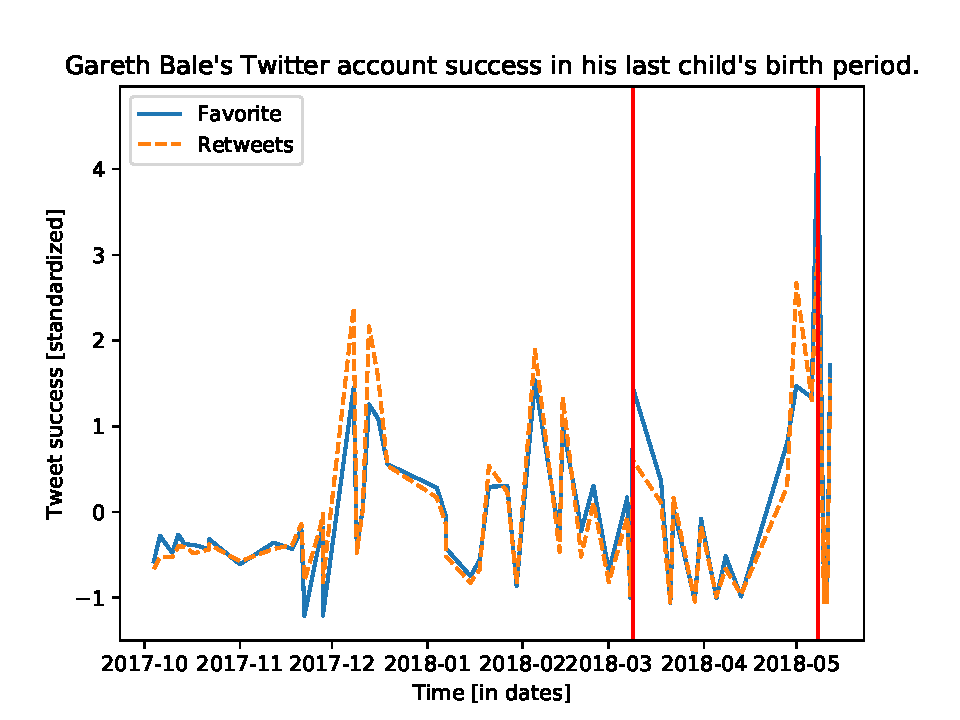
\includegraphics[width=%
0.8\textwidth]{img/bale}
\caption{The success -- number of likes and shares -- of the posts standardized and plottet over time. The two vertical lines represent the moments when the user talks about a life event. In both cases, the success is very high.}
\label{fig:bale}
\end{figure}

This last function has the goal to analyze the user's timeline to discover a life event in it. Since a life event is something important and rare into a user's life, the assumption is that also in her social life her behaviour is different when the event is approaching or is in progress. For this reason some unusual patterns, related to the life event itself or to the average success of the posts, are searched for. The idea is that a user does not publishes contents about, for examples, a new baby, very usually, but only when something important is about to happen. In addition to that, according to \cite{dickinson2015identifying}, a post about a new baby announcement gets probably more feedbacks compared to a normal post, such as congratulation messages. As also shown in Figure~\ref{fig:bale}, when the user talks about a life event, the success of her post tends to be high. The detection of a life event is based on these routine changes, which can be various: a slow but constant increase of interest before the event, or a sudden peak when the event is happening. In general, the relative frequency of activities related to the life event itself is monitored.

At this point, a timeline is composed by a list of post, each one with the probability of being about the life event, and with the other metadata, like date of publication and post success. Let $p$ be the probability given by the classifier about a post, that post is considered related to the life event if $ p > p_1$. If the previous condition is false, but $p_2 \leq p \leq p_1 $, the post success is taken into consideration to decide if the post is about the life event: let $n$ the number of post of a user, and
\[
\mu_\text{likes} = \frac{1}{n} \sum_{i=1}^n post_i.likes \quad \mu_\text{shares} = \frac{1}{n} \sum_{i=1}^n post_i.shares \quad \mu_\text{sentiment} = \frac{1}{n} \sum_{i=1}^n post_i.sentiment
\]
the average of likes, shares and sentiment score among all the user's post. If 
\begin{gather}
\label{avgs}
post.likes > \mu_\text{likes} \land post.shares > \mu_\text{shares} \land post.sentiment > \mu_\text{sentiment}
\end{gather}
the post is considered related to the life event, otherwise no.

For each day $d$ the user has been active on social media (those days in which the user published something), the frequency $f$ is computed as follows:
\begin{gather}
f(d) = \frac{r(d)}{all(d)}
\label{freq}
\end{gather}
where $r(d)$ is the number of posts related to the life event written the day $d$, and $all(d)$ is the count of all posts published the day $d$.

Of course, the timeline is already targeted with the life event taken into consideration. In other words, the life event to monitor is chosen in the previous steps: at this point the timeline is labelled only for a single life event. Once the frequency has been computed for every day, it can be plotted over time, and at the moment $f$ passes a given threshold $\alpha$, the life event is begun. When a minimum number of days $\beta$ in which $f(t) > \alpha$ are found, the life event can be considered as detected. By the time in $\gamma$ days there are no \emph{active days}, the life event can be seen as over.

As input, is expected a list of probabilities, each one with a timestamp, that represents the user's timeline in function to a life event.

As output, a list with time ranges in which the life events have been detected is expected (this range can be composed by the date of the first and the last post related to the life event). Of course, the user may have not lived the life event, so in this case the list will be empty.

There are several parameter for this phase: 
\begin{itemize}
\item a pair of probabilities $p_1$ and $p_2$ to consider a post directly related with the life event, or to check post success to take that decision. By default, $p_1 = 0.6$ and $p_2 = 0.4$.
\item the threshold $\alpha$ for the frequency $f$ over which the life event is considered as started.
\item $\beta$, the minimum number of \emph{active posts} to consider a life event detected. This parameter serves to correct any errors in post classification. In fact, is possible that a text or an image is misclassified: using this parameter is possible to avoid single and isolated errors.
\item $\gamma$, the maximum time between two \emph{active days} to consider them as related to the same life event. This parameter has the role to put an end to a detection, and consequently to split two consecutive life events.
\end{itemize}

\section{Interfaces of the components}
\label{sec:apis}
In this section the API of each component are presented. Internal APIs are very important to allow system scalability and to facilitate any future changes to the logic or to the functionalities. Firstly, some data types used inside the system are formalized, and secondly, the API are listed.

The first data type represents a \emph{user}, which is a subject of a computation. The object \texttt{User} is so composed:

\begin{center}
\label{tab:user}
\begin{tabular}{lll}
\hline
User & & \\
\hline
\textbf{Integer} & userID & \%The ID of the user inside the system. It is a unique number \\
\textbf{String} & name & \%The name of the user \\
\textbf{SocialNetworkUser}[] & socials & \%Array of social networks in which she's registered in \\
\hline
\end{tabular}
\end{center}

where a \texttt{SocialNetworkUser} object is so composed:

\begin{center}
\label{tab:social}
\begin{tabular}{lll}
\hline
SocialNetworkUser & & \\
\hline
\textbf{Integer} & socialID & \%The ID of the user inside this specific social network \\
\textbf{String} & name & \%The name of the user in this social network \\
\textbf{Integer} & from & \%ID of the first post downloaded \\
\textbf{Integer} & to & \%ID of the last post downloaded \\
\hline
\end{tabular}
\end{center}

The fields \emph{from} and \emph{to} are needed to understand where to begin a download request. Finally, the concept of \emph{post} is now formalized in an object call \texttt{Post}: it includes all the useful data for this purpose, such as date of creation, number of likes and shares, sentiment score, entity and topic sets and the probability to be about a life event. At the beginning of the analysis, many of these attributes are empty, and each logical step adds a piece of information. Each post is uniquely identified by the couple (ID, social networks).

\begin{center}
\label{tab:post}
\begin{tabular}{lll}
\hline
Post & & \\
\hline
\textbf{Integer} & postID & \%The ID of the post in the social network\\
\textbf{String} & socialNetwork & \%The social network from where the post comes from \\
\textbf{User} & author & \%The author of the post \\
\textbf{Date} & created & \%The creation date of the post \\
\textbf{Integer} & likes & \%Number of likes received \\
\textbf{Integer} & shares & \%Number of shares \\
\textbf{Float} & sentiment & \%Sentiment score \\
\textbf{Set} & entities & \%Set of strings representing the entities found in post text or images \\
\textbf{Set} & topics & \%Set of strings representing the topics found in post text or images \\
\textbf{Float} & probability & \%Probability of the post to be about a life event \\
\hline
\end{tabular}
\end{center}

Now the API of the four logical component are presented. Each one can be seen as a web interface that accepts and returns JSON objects. Every time that an object described just above here is used, only the parameters to uniquely identify an instance of these objects are passed or returned as parameters. For example, only a \texttt{userID} is used to indicate an \texttt{User} instance.

\subsection{Collector API}
The collector needs a \texttt{User} instance to which fetch her contents online, and a count that indicates how many activities to download from each social network.

Input:
\begin{itemize}
\item \texttt{userID}, Integer.
\item \texttt{count}, Integer.
\end{itemize}

Output:
\begin{itemize}
\item a list of \texttt{Post} identified by \texttt{postID} and \texttt{socialNetwork}.
\end{itemize}

Below an example of input and output.
\begin{multicols}{2}
\begin{Verbatim}
//input
{
  "userID": 2565227499,
  "count": 200
}


//output
[
  {
    "postID": 667069250268479488,
    "socialNetwork": "Twitter"
  }
]
\end{Verbatim}
\end{multicols}

\subsection{Entity extraction API}
The extractor needs a \texttt{Post} instance to which extract entities, and returns the same instance enriched.

Input and output are the same:
\begin{itemize}
\item \texttt{postID}, Integer.
\item \texttt{socialNetwork}, String.
\end{itemize}

Below an example in JSON format. Both input and output are the same.

\begin{Verbatim}
{
  "postID": 667069250268479488,
  "socialNetwork": "Twitter"
}
\end{Verbatim}

\subsection{Post classifier API}
The classifier takes a life event on which the classification is based, and a list of \texttt{Post} instances and adds the attributes \texttt{probability}, that indicates the probability with which each post is about the life event. It returns the same instances with the probability added.

Input:
\begin{itemize}
\item \texttt{lifeEvent}, String.
\item a list of \texttt{Post}, each one identified by \texttt{postID} and \texttt{socialNetwork}.
\end{itemize}

Output:
\begin{itemize}
\item a list of \texttt{Post}, each one identified by \texttt{postID} and \texttt{socialNetwork}.
\end{itemize}

Below an example of input and output.
\begin{multicols}{2}
\begin{Verbatim}
//input
{
  "lifeEvent": "Having children",
  "posts": [
   {
     "postID": 667069250268479488,
     "socialNetwork": "Twitter"
   }
  ]
}
//output
[
  {
    "postID": 667069250268479488,
    "socialNetwork": "Twitter"
  }
]



\end{Verbatim}
\end{multicols}

\subsection{Timeline analyzer API}
The timeline analyzer needs a list of \texttt{Post}, which represents the user's \emph{timeline}. Each one has to have a probability of being about a life event. It returns a list of pairs of dates, each one indicating the beginning and the end of a life event found in the timeline. The list can be empty.

Input:
\begin{itemize}
\item a list of \texttt{Post}, each one identified by \texttt{postID} and \texttt{socialNetwork}.
\end{itemize}

Output:
\begin{itemize}
\item a list of pairs of dates.
\end{itemize}

An example of input and output is presented below.
\begin{multicols}{2}
\begin{Verbatim}
//input
[
  {
    "postID": 667069250268479488,
    "socialNetwork": "Twitter"
  }
]
//output
[
  {
    "from": "2018-3-8",
    "to": "2018-5-24"
  }
]
\end{Verbatim}
\end{multicols}

\section{The detection algorithm}
\label{sec:alg}

In this part the detection algorithm, whose logic was previously explained in Section~\ref{sec:computationperformer}, is defined in pseudocode. It is assumed that all the parameters previously highlighted in Section~\ref{sec:computationperformer} are defined, and that all the three previous logical steps have already been executed. Let $n$ be the number of posts in the timeline taken into analysis, and let the data type \texttt{Post} be defined as in Section~\ref{tab:post}.

The algorithm is composed by two main parts. In the first part, the goal is to compute the average number of likes and shares received by the user among her posts, and the average sentiment score. After that, all the posts are grouped by date of publication, creating a dictionary with the days in which the user has published something as keys ($k$ indicates a single key), and as values the tuple (posts related with the life event on day $k$, all posts on day $k$). This is explained in Algorithm~\ref{freq_computing}.

\begin{algorithm}
\caption{Compute the relative frequency of activities related to the life event.}
\label{freq_computing}
\begin{algorithmic}[1]
\Require posts must be sorted by date
\Function{computeFrequency}{Post[] posts}
\State $AVGLikes \gets \frac{1}{n} \sum_{i=1}^n p_i.likes $
\State $AVGShares \gets \frac{1}{n} \sum_{i=1}^n p_i.shares $
\State $AVGSentiment \gets \frac{1}{n} \sum_{i=1}^n p_i.sentiment$
\State $frequencies \gets \{\}$
\State $count \gets 0$
\State $total \gets 0$
\For{$i \gets 1 \text{ to } n$}
	\State $total \gets total + 1$
	\If{$posts[i].probability > p_1$}
		\State $count \gets count + 1$
	\ElsIf{$posts[i].probability \geq p_2 \land posts[i].likes > AVGLikes \land posts[i].shares > AVGShares \land posts[i].sentiment > AVGSentiment$}
		\State $count \gets count + 1$
	\EndIf
	\If{$i = n \lor posts[i].created \ne posts[i + 1].created$}
		\State $frequencies[posts[i].created] \gets (count, total)$
	\EndIf
\EndFor
\Return $frequencies$
\EndFunction 
\end{algorithmic}
\end{algorithm}

For each day $k$, $count$ and $total$ are computed, which represent the number of posts related to the life event and the total number of post on that day respectively. At line 10 the decision to trust the classification directly is taken. In case it is not trusted, the condition at line 12 checks whether the probability is greater or equal than $p_2$ and if number of likes, shares and sentiment score are all over the average of the user, the post is considered related to the life event, as explained in Formula~\ref{avgs}. The last condition at line 14 is to understand whether a post is the last one for a day: this happens when the current post is the last one in the collection, or when the next one has a different date of creation.

In the second part, the dictionary created in the first part is analyzed, computing for each day $k$ the frequency of activeness as in Formula~\ref{freq} and analyzing this latter to understand if there are significant changes on it. This is explained in Algorithm~\ref{decision}. Also here it is assumed that the days in the dictionary are analyzed in increasing order.

\begin{algorithm}
\caption{Decide whether a user has lived a life event}
\label{decision}
\begin{algorithmic}[1]
\Function{DetectLifeEvents}{frequencies}
\State $start \gets today()$
\State $end \gets \perp$
\State $count \gets 0$
\State $found \gets \{\}$
\ForAll{$k \in \text{frequencies}$}
	\State $f \gets \frac{\text{frequencies}[k].count}{\text{frequencies}[k].total}$
	\If{$f > \alpha$}
		\If{$k < start$}
			\State $start \gets k$
			\State $end \gets k$
		\EndIf
		\If{$(k - end) < \gamma$}
			\State $end \gets k$
			\State $count \gets \text{frequencies}[k].count$
		\Else
			\If{$count \geq \beta$}
				\State $found \gets found \cup \{(start, end)\}$
			\EndIf
			\State $start \gets k$
			\State $end \gets k$
			\State $count \gets 1$
		\EndIf
	\EndIf
\EndFor
\If{$count \geq \beta \land end \ne \perp$}
	\State $found \gets found \cup \{(start, end)\}$
\EndIf
\Return $found$
\EndFunction
\end{algorithmic}
\end{algorithm}

The symbol $\perp$ represents a null type. The idea is to find some time intervals that represent a life event, each one recognized by a $start$ and an $end$. For each day in which the user published something, the relative frequency $f$ is computed (at line 7) as shown in Formula~\ref{freq}. If $f$ is greater than the threshold $\alpha$ and it is the very first day encountered, $start$ will point to it. For every other following day $k$ in which $f > \alpha$ and $k$ comes less than $\gamma$ days later than the current $end$, $end$ is overwritten, and putted equal to $k$. When an active day is too far from the last active day, the conditions to add a life event are checked (line 16): if at least $\beta$ active posts were previously found, the life event from $start$ to $end$ is added, and these variables are resetted to detect another interval. In the end, at line 21, is verified whether there is an interval left open, and in this case, if there are enough posts, a last life event is added.

The complexity of both Algorithms~\ref{freq_computing} and~\ref{decision} is $\Theta(n)$ in time, because each post is analyzed only once, in both functions. In case posts are not sorted by date, the computational cost will be dominated by the sorting procedure, becoming $\Theta(n \log n)$.

\section{Exposed APIs}
\label{sec:APIs}

In this section the user endpoint APIs offered by the system are defined. These interfaces are RESTful APIs, which expose the main resources available in the system: \texttt{User}, \texttt{Download Request} and \texttt{Computation}. For each resource, the possibilities to retrieve and create new instances are offered, and for the user resource is also possible to edit an instance. The structure of the \texttt{User} resource is described in Section~\ref{sec:apis}. A \texttt{Download Request} is meant to download user's contents from social media, and it is executed asynchronously, as explained in Section~\ref{sec:downloadqueues}. Finally, a \texttt{Computation} is an analysis on a user's timeline with a given life event, as described in Section~\ref{sec:alg}.

Each response has a field \texttt{"ok"} that indicates whether everything went well. In case an error occurs, the field \texttt{"error"} gives a human readable explanation of the error, while the HTTP status code indicates what kind of problem occurred (for example a 404 error in case the user requires a resources that doesn't exist).

The complete API specification can be found on Apiary:
\begin{center}
\url{lifeevents.docs.apiary.io}
\end{center}

